
%(BEGIN_QUESTION)

Hvilken motstand får størst spenningsfall når?
\vskip 10pt
a) $R_1=R_2=R_3$
\vskip 10pt
b) $R_2=(R_1+R_3)$
\vskip 10pt
b) $(R_1=R_3)>R_2$
\vskip 10pt

$$\includegraphics{i04874x01.eps}$$


\underbar{file i04874}
%(END_QUESTION)





%(BEGIN_ANSWER)


%(END_ANSWER)





%(BEGIN_NOTES)



%INDEX% Electronics review: series-parallel circuits

%(END_NOTES)


